% !TEX root = ../main.tex
\chapter{Related Work} \label{ch:reated_work}




























In this chapter, we give an overview of graph based algorithms
for image segmentation 

\section{Multicut}\label{sec:rw_multicut}

Segmentation is an important problem in computer vision as a first step
towards understanding an image. Many algorithms start with an over-segmentation
into superpixels, which are then clustered into ``perceptually meaningful''
regions.
Usually, the number of these regions is not known beforehand.

Recently, the multicut formulation~\cite{chopra_1993_mp}
(sometimes called \emph{correlation clustering}, \cite{bansal_2004_ml})
has become increasingly popular for unsupervised
image segmentation \cite{andres_2011_iccv,yarkony_2012_eccv,alush_2013_simbad}.

In this section we will give a brief overview of methods using multicut objectives
and will briefly introduce the multicut formulation.
The multicut and related work will be discussed extensively in \cref{ch:cgc} where
we propose a new solver for the such problems.

\paragraph{Problem Formulation:}
Given an edge-weighted region adjacency graph,
the problem is to find the segmentation which
minimizes the cost of the cut edges.
Therefore multicuts can be viewed as \emph{thresholding} w.r.t. close contours, while
naive thresholding will lead to inconsistencies 
(see \cref{fig:naive_thresholding} ).

Let $G=(V,E, \w)$ be a weighted region adjacency graph of
nodes $V$, representing superpixels,
and edges $E$.
%
The function $\w : E \rightarrow \mathbb{R}$ assigns a weight to each edge.
A positive weight expresses the desire that two adjacent nodes should
be merged, whereas a negative weight indicates
that these nodes should be separated into two different regions.
The \emph{multicut problem} can be written as a node labeling problem
\cite{bagon_2011_arxiv}:
%
\begin{align}
\argmin_{\Labels}
    \left\{
    \sum_{ e=(i,j) \in E}
        \w(e)
        \cdot \delta( \Labels_i \neq \Labels_j )
    \right\},
    \label{eq:multicut_primal_a}
\end{align}
%
where $\delta(a) = 1$ if $a$ is true and $0$ else.





\begin{figure}
\centering
\subfloat[Oversegmentation]{ \label{fig:naive_thresholding_a}
    \includegraphics[width=0.25\textwidth]{fig/andres/0.png}
}
\subfloat[Oversegmentation]{  \label{fig:naive_thresholding_b}
    \includegraphics[width=0.25\textwidth]{fig/andres/1.png}
}
\subfloat[Oversegmentation]{  \label{fig:naive_thresholding_c}
    \includegraphics[width=0.25\textwidth]{fig/andres/2.png}
}
\addtocontents{lof}{%
    \vspace{1cm}
    \protect\centerline{%
        \protect\includegraphics[width=.075\linewidth]{fig/andres/0.png}\hspace{0.2cm}
        \protect\includegraphics[width=.075\linewidth]{fig/andres/1.png}\hspace{0.2cm}
        \protect\includegraphics[width=.075\linewidth]{fig/andres/2.png} 
    }%
}%
\caption[Naive thresholding vs. multicuts]{
This figure has been taken from \cite{andres_2011_iccv} .
\Cref{fig:naive_thresholding_a} shows the oversegmentation of 
an image .
\Cref{fig:naive_thresholding_b} shows the result of naive thresholding..
Any inconsistent boundary is shown in red while consistent
boundaries are shown in yellow. 
\Cref{fig:naive_thresholding_c} shows the result with the multicut
constraints which lead to a meaningful segmentation.
} \label{fig:naive_thresholding}
\end{figure}


\citet{andres_2011_iccv} and \citet{kappes_2011_emmcvpr} use a
cutting plane approach where violated constraints are added
iteratively until no more violated constraints are found.


\begin{figure}
\centering
\subfloat[Superpixel Segmentation]{ \label{fig:mc_ineq_0}
    \includegraphics[width=0.4\textwidth]{fig/andres/ineq_0.pdf}
}
\subfloat[Corresponding Graph]{ \label{fig:ineq_1}
    \includegraphics[width=0.4\textwidth]{fig/andres/ineq_1.pdf}
}
\addtocontents{lof}{%
    \vspace{1cm}
    \protect\centerline{%
        \protect\includegraphics[width=.075\linewidth]{fig/andres/ineq_0.pdf}\hspace{0.2cm}
        \protect\includegraphics[width=.075\linewidth]{fig/andres/ineq_1.pdf}
    }%
}%
\caption[Violated multicut constraints]{
This figure has been taken from \cite{andres_2011_iccv} .
\Cref{fig:mc_ineq_0} shows the oversegmentation of 
an image .
\Cref{fig:mc_ineq_1} shows the corresponding graph.
} \label{fig:mc_ineq}
\end{figure}




\section{Hierarchical Clustering}\label{sec:rw_hc}

%%%%%%%%%%%%%%%%%%%%%
%dendrogram
%%%%%%%%%%%%%%%%%%%%%%
\begin{figure}
    \centering
    \subfloat[Bottom-Up: Nodes are merged with increasing time]{\label{fig:hc_bottom_up}
        {
            \begin{tikzpicture}[sloped]
                \node (a)    at (-6,0)      {a};
                \node (b)    at (-5,0)      {b};
                \node (c)    at (-4,0)    {c};
                \node (d)    at (-3,0)     {d};
                \node (e)    at (-2,0)       {e};

                \node (ab)   at (-5.5,1)    {};
                \node (cd)   at (-3.5,1)    {};
                \node (cde)  at (-2.75,2)       {};
                \node (all)  at (-4,3)    {};
                
                \node (root) at (-4,4) {root}; 

                \draw (a) |- (ab.center);
                \draw (b) |- (ab.center);
                \draw (c) |- (cd.center);
                \draw (d) |- (cd.center);
                \draw (e) |- (cde.center);
                \draw (cd.center) |- (cde.center);
                \draw (ab.center) |- (all.center);
                \draw (cde.center) |- (all.center);
                \draw (all.center) |- (root.center);

                \draw[->,-triangle 60] (-7,0) -- node[above]{time} (-7,4);
            \end{tikzpicture}
        }
    }\hspace{2cm}
    \subfloat[Top-Down: Nodes are divided with increasing time]{\label{fig:hc_top_down}
        {
            \begin{tikzpicture}[sloped]
                \node (a)    at (-6,0)      {a};
                \node (b)    at (-5,0)      {b};
                \node (c)    at (-4,0)    {c};
                \node (d)    at (-3,0)     {d};
                \node (e)    at (-2,0)       {e};

                \node (ab)   at (-5.5,1)    {};
                \node (de)   at (-2.5,1)    {};
                \node (cde)  at (-3.25,2)       {};
                \node (all)  at (-4,3)    {};
                
                \node (root) at (-4,4) {root}; 

                \draw (a) |- (ab.center);
                \draw (b) |- (ab.center);
                \draw (c) |- (cde.center);
                \draw (d) |- (de.center);
                \draw (e) |- (de.center);        
                \draw (de.center) |- (cde.center);
                \draw (ab.center) |- (all.center);
                \draw (cde.center) |- (all.center);
                \draw (all.center) |- (root.center);

                \draw [->,-triangle 60] (-7,4) -- node[below,align=center]{time} (-7,0);
            \end{tikzpicture}
        }
    }
    \addtocontents{lof}{%
    \vspace{1cm}
    \protect\centerline{%
    \protect\includegraphics[width=.2\linewidth]{fig/thump/dendro.png}
    }%
    }%
    \caption[Bottom-up vs. top-down hierarchical clustering]{
        Describe the difference between both
    }
    \label{fig:hc_bottom_up_top_down}
\end{figure}


Hierarchical clustering techniques have been successfully used
in computer vision since decades \citep{ohlander_1978_cgip,forsyth_2002_book,arbelaez_2006_cvpr,iglesias_2013,morel_1995_book}.

The method  of \citet{ohlander_1978_cgip} is an example for \emph{top-down} clustering,
where all pixel start in one single cluster. Each cluster is recursively divided 
into  more clusters. The method proposed in \cref{ch:cgc} has a strong connection to
\emph{top-down} clustering.
\citet{arbelaez_2006_cvpr} and \citet{iglesias_2013} use the bottom-up approach 
also called \emph{agglomerative clustering}, where 
adjacent nodes in a graph are merged iteratively to create 
a set of nested segmentations.


Such a hierarchy of clusters can be visualized as a dendrogram (see \cref{fig:hc_bottom_up_top_down} ).
The dendrogram can be interpreted as a tree where each node represents a
region in the image.
The leafs in the tree are the atomic units of the image (e.g. pixel,superpixels, supervoxel)
and the root note is the entire scene itself (e.g. the complete image / graph).

There are a few difference between classic unstructured agglomerative clustering
\citep{florek_1951,sokal_1958_science_bulletin,ward_63_jasa}
and agglomerative clustering on graph data structures \citep{arbelaez_2006_cvpr,iglesias_2013,morel_1995_book}, 
e.g. grid-graphs and region adjacency graphs\citep{vlachos_1993_csv}.
While in unstructured hierarchical clustering any pair of observations could be merged,
in the case of graph hierarchical clustering only adjacent nodes / regions can be merged.
In the literature this is also called ``hierarchical clustering with connectivity constraints''.


The main idea behind agglomerative clustering is very simple:

Initially, all observations start in a single cluster. 
Next, cluster which have highest similarities / lowest distances will be merged.
Due to the merging, similarities will change and need to be updated
/ recomputed. Therefore  noisy initial features
will  become more informative .


\begin{table}
\begin{scriptsize}
\begin{tabular}{ |l|l|p{5cm}|}
    \hline 
    Euclidean Distance
        & $||a-b||_2 = \sqrt{\sum{ (a_i-b_i })^2 } $
        & For low dimensional data \\  \hline 
    Squared Euclidean Distance
        & $||a-b||_2^2 = \sum{ (a_i-b_i })^2  $
        & For low dimensions data\\  \hline
    Manhattan Distance
        &  $||a-b||_1 = \sum{ |a_i-b_i |}  $
        & Multi purpose \\  \hline 
    Mahalanobis Distance 
        & $\sqrt{(a-b)S^-1(a-b)^T}$
        & ??? when to use \\  \hline 
    $\mathcal{X}^2$-Distance  
        &  $\frac{1}{2}\sum{  \frac{(a_i-b_i)^2}{a_i+b_i} }$
        & For histograms \\  \hline 
    Earth Mover  Distance          
        &  see \citet{levina_2001_iccv} 
        & For histograms \\  \hline 

\end{tabular}

\end{scriptsize}
\caption{
    An overview of the most common distances measurements and their main properties.
}\label{tab:hc_distance_types}
\end{table}



\begin{table}
\begin{scriptsize}
\begin{tabular}{ |l|l|p{5cm}|}
    \hline
    Average Linkage \citep{sokal_1958_science_bulletin}           
        & $d_{al}(C_a,C_b) = \frac{1}{|C_a||C_b|} \sum _{a \in C_a} \sum_{b \in C_b} d(a,b) $ 
        & \scriptsize Prefers clusters with same variance \cite{sokal_1958_science_bulletin} \\ \hline

    Single Linkage \citep{florek_1951}            
        & $d_{sl}(C_a,C_b) =  \min\{d(a,b) : a \in C_a, b \in C_b\}$ 
        & Nice theoretic properties \citep{hartigan_1981_jjamstat,milligan_1980_psycho}, can lead
          to very irregular shaped clusters \\ \hline
    Complete Linkage \citep{sorensen_1948}         
        & $d_{cl}(C_a,C_b) =  \max\{d(a,b) : a \in C_a, b \in C_b\}$ 
        & Prefers clusters with same diameter \citep{milligan_1980_psycho} \\ \hline
    Centroid Distance         
        & $d_{cd}(C_a,C_b) =  d(\bar{C}_a,\bar{C}_b) $ 
        & Robust w.r.t. outliers \citep{milligan_1980_psycho} \\ \hline
    Wards Minimum Variance \citep{ward_63_jasa}
        & $d_{wmv}(C_a,C_b) = \frac{ d(\bar{C}_a,\bar{C}_b)}{ \frac{1}{|C_a|} + \frac{1}{|C_b|} } $ 
        & Prefers clusters with same size, is sensible to outliers \citep{milligan_1980_psycho} \\ \hline
\end{tabular}

\end{scriptsize}

\caption{
    An overview of the most common cluster distances linkages and their main properties.
}\label{tab:hc_linkage_types}
\end{table}


The definition of a specific distance betweens clusters is very crucial, 
but does strongly depend on the application.
In \cref{tab:hc_distance_types} is a short overview of most common distance
types and in   \cref{tab:hc_linkage_types} is a  brief overview 
of cluster distance linkage types.








\iffalse
\begin{tikzpicture}[scale=  1,every node/.style={minimum size=1cm},on grid]
        
    %slanting: production of a set of n 'laminae' to be piled up. N=number of grids.
    

    %%%%%%%%%%%%%%%%%%%%%%%%%%%%%%%%%%%%%%%%%%%%%%%%%%%%%%%%%%%%%%%
    % 0 bottom layer
    %%%%%%%%%%%%%%%%%%%%%%%%%%%%%%%%%%%%%%%%%%%%%%%%%%%%%%%%%%%%%%%%
        
    \begin{scope}[yshift=0,every node/.append style={yslant=0.5,xslant=-1},yslant=0.5,xslant=-1]
        \draw[-latex,thick] (-0.17,3.21/2) node[right]{\includegraphics[width=4.82cm]{fig/12074/0.png}};
        \draw[black,very thick] (0,0) rectangle (4.81,3.21);
    \end{scope}

    \begin{scope}[yshift=60*1,every node/.append style={yslant=0.5,xslant=-1},yslant=0.5,xslant=-1]
        \draw[-latex,thick] (-0.17,3.21/2) node[right]{\includegraphics[width=4.82cm]{fig/12074/2.png}};
        \draw[black,very thick] (0,0) rectangle (4.81,3.21);
    \end{scope}

    \begin{scope}[yshift=60*2,every node/.append style={yslant=0.5,xslant=-1},yslant=0.5,xslant=-1]
        \draw[-latex,thick] (-0.17,3.21/2) node[right]{\includegraphics[width=4.82cm]{fig/12074/4.png}};
        \draw[black,very thick] (0,0) rectangle (4.81,3.21);
    \end{scope}

    \begin{scope}[yshift=60*3,every node/.append style={yslant=0.5,xslant=-1},yslant=0.5,xslant=-1]
        \draw[-latex,thick] (-0.17,3.21/2) node[right]{\includegraphics[width=4.82cm]{fig/12074/6.png}};
        \draw[black,very thick] (0,0) rectangle (4.81,3.21);
    \end{scope}

    \begin{scope}[yshift=60*4,every node/.append style={yslant=0.5,xslant=-1},yslant=0.5,xslant=-1]
        \draw[-latex,thick] (-0.17,3.21/2) node[right]{\includegraphics[width=4.82cm]{fig/12074/8.png}};
        \draw[black,very thick] (0,0) rectangle (4.81,3.21);
    \end{scope}


    \draw[->,-triangle 60] (-3,0) -- node[above]{time} (-3,4);

    %%%%%%%%%%%%%%%%%%%%%%%%%%%%%%%%%%%%%%%%%%%%%%%%%%%%%%%%%%%%%%%
    % 0 bottom layer
    %%%%%%%%%%%%%%%%%%%%%%%%%%%%%%%%%%%%%%%%%%%%%%%%%%%%%%%%%%%%%%%%
    \draw[-latex,thick] (6.2,2) node[right]{$\mathsf{over-segmentation}$}
         to[out=180,in=90] (4,2);
         
         
         
    %%%%%%%%%%%%%%%%%%%%%%%%%%%%%%%%%%%%%%%%%%%%%%%%%%%%%%%%%%%%%%%
    % 1 layer
    %%%%%%%%%%%%%%%%%%%%%%%%%%%%%%%%%%%%%%%%%%%%%%%%%%%%%%%%%%%%%%%%
    
    \draw[-latex,thick] (6.2,5.5) node[right]{$\mathsf{Region adjacency graph 1}$}
         to[out=180,in=90] (4,5.5);
\end{tikzpicture}
\fi







In the case of graph hierarchical clustering, informative features
can also be attached to the edges of the graph.
Unsupervised edge detectors as gPb \citep{marie_2008_cvpr}  or learned
edge detectors \cite{dollar_2013_iccv}  can be used to boost performance
of agglomerative clustering \citep{arbelaez_2006_cvpr,iglesias_2013}.



\citet{ arbelaez_2006_cvpr} uses $\Omega \in \mathbb{R}^2$ as image domain.
$P_0$ is the inital partition of $\Omega$ and define a
\emph{hierarchical segmentation operator} (HSO) which
assignes a partiton $P_\lambda$ given the inital partiton and
a scale parameter $\lambda$.
Furthermore the follwing properties must be fullfilled for an HSO.  


\begin{align} 
P_{\lambda}  =  P_0 ,\hspace{0.5cm}  \forall \lambda \leq 0  \label{eq:ucm_hco_eq_0} \\ 
\exists \lambda_1 \in \mathbb{R}^+  : P_{\lambda}  =  \{ \Omega \} ,\hspace{0.5cm} \forall \lambda \geq \lambda_1  \label{eq:ucm_hco_eq_1} \\
\lambda < \lambda'  \rightarrow  P_{\lambda} \sqsubseteq   P_{\lambda'} \label{eq:ucm_hco_eq_2}
\end{align}


\Cref{eq:ucm_hco_eq_0} and \cref{eq:ucm_hco_eq_1}  give $\lambda$ a range.
\Cref{eq:ucm_hco_eq_2} ensures that the segmentations are nested.
They define the \emph{salience} of a contour as the scale $\lambda$ where
the contour disappears (see \cref{fig:ucm_visu} and \cref{fig:ucm_saliency} )
Thresholding the saliency map will lead to closed contours.
As a consequence, the a complete hierarchical segmentation
generated by a HSO can be encoded in the saliency map.


\citet{iglesias_2013} try to improve segmentation with
the use of agglomerative clustering combined with machine learning.
Their main idea is to combine training data and features at multiple scales
which are generated during the region merging process.
They show that they can outperform the classic approach
of flat learning.


\begin{figure} 
    \begin{center}
        \subfloat[$K_0$]{ \label{fig:ucm_k0}
            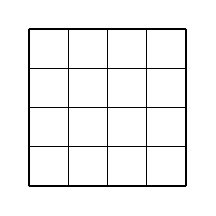
\begin{tikzpicture}
                \draw[step=0.5,black,thin] (0.0,0.0) grid (2,2);
                \draw[step=2,black,thick] (0.0,0.0) grid (2,2);
            \end{tikzpicture}
        }
        \hspace{0.5cm}
        %
        %
        %
        \subfloat[$K_1$]{ \label{fig:ucm_k1}
            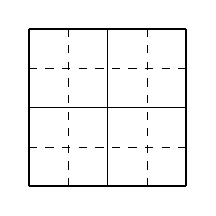
\begin{tikzpicture}
                \draw[step=0.5,black,very thin,dashed] (0.0,0.0) grid (2,2);
                \draw[step=1,black,thin] (0.0,0.0) grid (2,2);
                \draw[step=2,black,thick] (0.0,0.0) grid (2,2);
            \end{tikzpicture}
        }
        \hspace{0.5cm} 
        %
        %
        %
        \subfloat[$K_2$]{\label{fig:ucm_k2}
            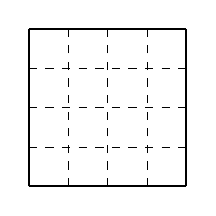
\begin{tikzpicture}
                \draw[step=0.5,black,very thin,dashed] (0.0,0.0) grid (2,2);
                \draw[step=2,black,thick] (0.0,0.0) grid (2,2);
            \end{tikzpicture}
        }
        \hspace{0.5cm}
        %
        %
        %
        \subfloat[$\mathcal{C}(\Upsilon) $]{ \label{fig:ucm_saliency}
            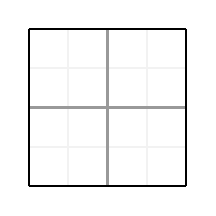
\begin{tikzpicture}
                \draw[step=0.5,black!5,thick] (0.0,0.0) grid (2,2);
                \draw[step=1,  black!40,thick] (0.0,0.0) grid (2,2);
                \draw[step=2,black,thick] (0.0,0.0) grid (2,2);
            \end{tikzpicture}
        }
        \hspace{0.5cm}
        %
        %
        %
        \subfloat[$\mathcal{C}(\Upsilon) $]{ \label{fig:ucm_saliency_3d}
            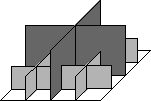
\includegraphics[width=0.2\textwidth]{fig/ucm3d.pdf}
        }
    \end{center}
    \addtocontents{lof}{%
    \vspace{1cm}
    \protect\centerline{%
        \protect\includegraphics[width=.2\linewidth]{fig/thump/ucm.png} 
    }%
    }%
    \caption[Ultra metric contour map saliency]{
        \Cref{fig:ucm_k0} shows the an $4x4$ grid graph which servers as initial segmentation $K_0$.
        \Cref{fig:ucm_k1} shows the segmentation $K_0$ after the contraction of a few edges.
        Contracted edges are showed dashed.
        \Cref{fig:ucm_k2} shows the graph after all edges have been contracted.
        \Cref{fig:ucm_saliency} shows the saliency $\mathcal{C}$ of the contour $\Upsilon$ of the contours.
        In \cref{fig:ucm_saliency_3d} the saliency from \ref{fig:ucm_saliency} as a 3D visualization.
        This figure is very much inspired from a figure showed in \citep{arbelaez_2006_cvpr}.
    }\label{fig:ucm_visu}
\end{figure}









\section{MST Methods}\label{sec:rw_mst_methods}


Discuss the method from \citet{felzenszwalb_2004_ijcv}.


Discuss the method from \citet{Straehle_k-smallestspanning}.


\section{Graph Cut and Energy Based Methods}

\subsection{Graph Cut}

\subsection{QPBO}

\subsection{Multilabel Methods}

    cite all multilabel methods from opengm benchmark


\section{Random Walker}\label{sec:rw_random_walker}



\section{Watershed Methods}\label{sec:rw_watershed_methods}

The idea of watersheds has been introduced by \citet{beucher_1979_workshop}.

Other watersheds \citep{vinent_1991_pami,najman_1994_sp,roerdink_2000_finf,bertrand_2005_jmiv,cousty_2009_pami}.


The watershed algorithm can be often described with the following analogy:

\paragraph{Water Flooding:} A grayscale  image can be interpreted as hight map (see \cref{fig:ws_2d_map}, \cref{fig:ws_2d_map3d}).
The water level is raised as shown in \cref{fig:ws_a} - \cref{fig:ws_f}.
A watershed is wherever the water of two adjacent valleys is meeting (see \cref{fig:ws_e},\cref{fig:ws_f} and \cref{fig:ws_2d_lines}).


% watersheds illustrated
\begin{figure}
    \centering
    \subfloat[1d Image Data]{ \label{fig:ws_a}
        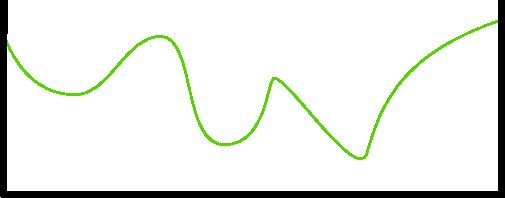
\includegraphics[width=0.25\textwidth]{fig/ws_no_no.pdf}
    }
    \hspace{0.5cm}
    \subfloat[Local minima]{  \label{fig:ws_b}
        \includegraphics[width=0.25\textwidth]{fig/ws_no.pdf}
    }
    \hspace{0.5cm}
    \subfloat[flooding starts]{  \label{fig:ws_c}
        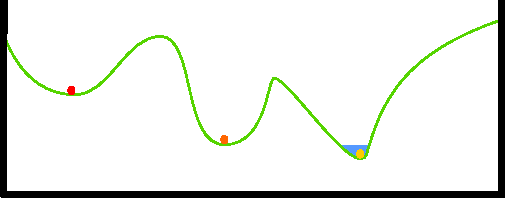
\includegraphics[width=0.25\textwidth]{fig/ws3.pdf}
    }
    \\
    \subfloat[flooding]{  \label{fig:ws_d}
        \includegraphics[width=0.25\textwidth]{fig/ws2.pdf}
    }
    \hspace{0.5cm}
    \subfloat[watershed 1]{  \label{fig:ws_e}
        \includegraphics[width=0.25\textwidth]{fig/ws1.pdf}
    }
    \hspace{0.5cm}
    \subfloat[watershed 2]{ \label{fig:ws_f}
        \includegraphics[width=0.25\textwidth]{fig/ws0.pdf}
    }
    \\ % 2D Watersheds
    \subfloat[$ $]{ \label{fig:ws_2d_map}
        \includegraphics[height=0.26\textwidth]{fig/ws2d0.png}
    }
    \hspace{0.1cm}
    \subfloat[$ $]{ \label{fig:ws_2d_map3d}
        \includegraphics[height=0.26\textwidth]{fig/ws2d1.png} 
    }
    \hspace{0.1cm}
    \subfloat[$ $]{ \label{fig:ws_2d_lines}
        \includegraphics[height=0.26\textwidth]{fig/ws2d2.png}
    }

    \addtocontents{lof}{%
        \vspace{1cm}
        \protect\centerline{%
            \protect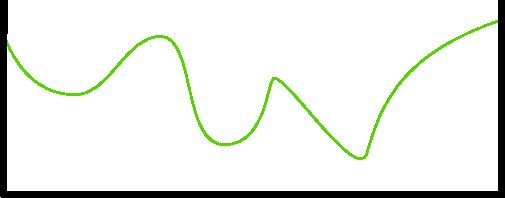
\includegraphics[width=.075\linewidth]{fig/ws_no_no.pdf}  \hspace{0.2cm}
            \protect\includegraphics[width=.075\linewidth]{fig/ws_no.pdf}\hspace{0.2cm}
            \protect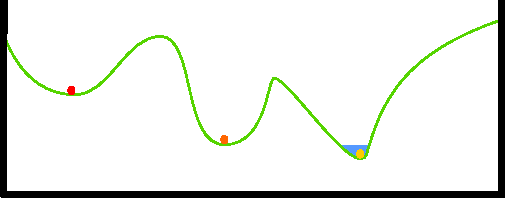
\includegraphics[width=.075\linewidth]{fig/ws3.pdf} 
        }%
        \vspace{0.2cm}
        \protect\centerline{%
            \protect\includegraphics[width=.075\linewidth]{fig/ws2.pdf}  \hspace{0.2cm}
            \protect\includegraphics[width=.075\linewidth]{fig/ws1.pdf} \hspace{0.2cm}
            \protect\includegraphics[width=.075\linewidth]{fig/ws0.pdf}%
        }%
        \vspace{0.2cm}
        \protect\centerline{%
            \protect\includegraphics[height=.075\linewidth]{fig/ws2d0.png}  \hspace{0.2cm}
            \protect\includegraphics[height=.075\linewidth]{fig/ws2d1.png} \hspace{0.2cm}
            \protect\includegraphics[height=.075\linewidth]{fig/ws2d2.png}%
        }%
    }%
    \caption[Illustration of watershed flooding process]{ 
        Illustration of watershed flooding process.
        The water level raises, and the watersheds are at the positions where water from different catchment basins is meeting.
    } \label{fig:watersheds_1d}
\end{figure}





\citet{couprie_2011_pami} proposed an algorithm, \emph{power-watershed}, a generalization of \citep{RANDOM_WALKER, GRAPH_CUT,WATHERSHEDS,sinop_2007_iccv}.
They define the following model.
\begin{align}\label{eq:power_watershed}
\min_x \sum_{e_{ij} \in E}  w_{ip}^p |x_i-x_j|^q + \sum_{v_i } w_{Fi}^p |x_i|^q + \sum_{v_i } w_{Bi}^p |x_i-1|^q \\
s.t. \hspace{0.35cm} x(F)=1, \hspace{0.5cm} x(B)=0
\end{align}
Setting $p$ to 1 will lead to the methods proposed by \citet{sinop_2007_iccv}.
\Citet{allene_icv_2010} pointed out when $p=1$ and $q \rightarrow \infty$, solving
\cref{eq:power_watershed} is equivalent to applying a minimum spanning forest algorithm.




\citet{straehle_2011_miccai} proposed a watershed based method for interactive segmentation
of neural volume electron  microskopy images.
They show how a background prior be be efficiently integrated into watersheds,
and that this prior is beneficial for neuro data.
In addition \citet{straehle_2012_cvpr} proposed an uncertainty estimator for
guided interactive segmentation based on watersheds.




\section{Normalized Cuts}


